\section{Durchführung und Versuchsaufbau}

\subsection{Druckbereich 30 bis 1000 mBar}
\begin{figure}[H]
    \centering
    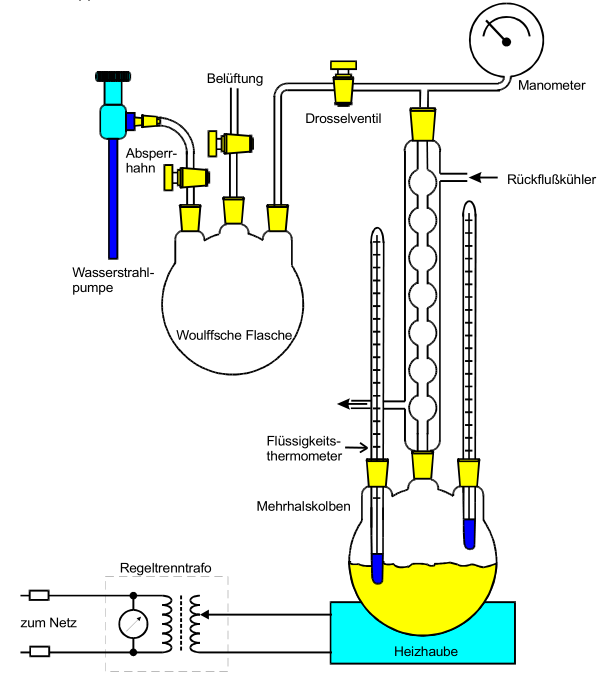
\includegraphics[width=0.55\textwidth]{images/Abbildung3.PNG}
    \caption{Der Versuchsaufbau für Drücke kleiner als 1 Bar \protect \cite{V203}.}
    \label{img:aufbau1}
\end{figure}
Für die Messung der Dampfdruckkurve wird die Apperatur aus der Abbildung \ref{img:aufbau1} verwendet. 
Den realen Aufbau findet man hier \ref{img:real1}. In dem Photo ist auf der linken Seite die Wasserstrahlpumpe in der Spüle. 
Der Absperrhahn, das Drosselventil und das Belüftungsventil sind direkt an der Woulffschen Flasche angeschlossen. Diese steht leicht 
links hinter der größeren Apparatur. Das linke Thermometer, welches die Temperatur der Flüssigkeit abliest, wird für diesen Versuch 
verwendet. Der Druck wird an dem digitalen Manometer rechts untem im Bild abgelsesen.\\
Um ein Vakuum für die Versuchsdurchführung zu erzeugen wird zunächst der Absperrhahn und das Drosselventil geöffnet und zusätzlich das 
Belülftungsventil geschlossen. Die Wasserstrahlpumpe wird nun solange angestellt bis sich ein konstanter Druck einstellt. 
Dieser Druck ist dabei, unter anderem, abhängig von der Wassertemperatur.\\
Bevor nun die Wasserstrahlpumpe abgeschaltet wird müssen der Absperrhahn und das Drosselventil geschlossen werden. 
Als nächstes wird nun die Heizhaube eingeschaltet und gleichzeitig dafür gesorgt, dass Kühlflüssigkeit durch den Rückflusskühler fließt. 
Falls die Substanz nach ein wenig Zeit nicht anfängt zu sieden wird noch einmal das Drosselventil geöffnet um den Druck innerhalb des Gefäßes weiter zu senken.\\
Anschließend wird bei laufender Heizung die Siedetemperatur und der Dampfdruck im Druckbereich $\SI{30}{\milli\bar}$ bis $\SI{1000}{\milli\bar}$ 
in fünfziger Schritten jeweils mit den Messgeräten gemessen. Damit höhere Temperaturen erreicht werden können 
muss nach einer Weile der Durchfluss der Kühlflüssigkeit reduziert werden, bis die Kühlflüssigkeit nur noch tropft.
\subsection{Druckbereich 1 bis 15 Bar}
\begin{figure}[H]
    \centering
    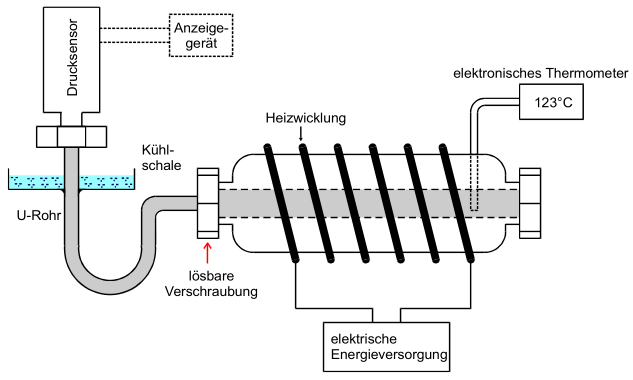
\includegraphics[width=0.55\textwidth]{images/Abbildung4.PNG}
    \caption{Der Versuchsaufbau für den Messbereich von 1 bis 15 Bar \protect \cite{V203}.}
    \label{img:aufbau2}
\end{figure}
Die Dampfdruckkurve für Drücke im Bereich von $\SI{1}{\bar}$ bis $\SI{15}{\bar}$ wird mit Hilfe der Apperatur in \ref{img:aufbau2} bestimmt. 
Ihr reales Äquivalent findet man hier \ref{img:real1}.\\
Um den Versuch zu starten muss zunächst der Hohlraum vollständig mit destilliertem und entgastem Wasser befüllt sein.
Sobald die Ap­pa­ra­tur eingeschalten ist, wird während das Wasser nun langsam erhizt, 
die Siedetemperatur und der Sättigungsdampfdruck abgelesen. Der Druck wird in $\SI{1}{\bar}$ Schritten mit den jeweils zugehörigen Temperaturen vermessen. 
Es sollte dabei besonders beachtet werden, dass der Vollauschlag des Manometers nicht überschritten wird.  